\chapter{Conceitos Básicos} \label{conceitos}
	Este capítulo aborda conceitos fundamentais para a compreensão dos métodos de geração de imagens HDR e obtenção de nuvem de pontos, que serão abordados nos capítulos posteriores.
	
\section{Faixa Dinâmica} \label{conceitoFaixa}
    Cada imagem digital possui uma certa quantidade de bits para representação das cores de cada um de seus pixels. A maior parte das câmeras convencionais do mercado geram imagens com pixels que são representados por 8 bits em cada canal de cor, o que resulta numa faixa de 256 valores possíveis. Quando uma imagem possui esta faixa de representação de cores esta é chamada de imagem com baixa faixa dinâmica (em inglês, Low Dynamic Range - LDR) por possuir uma faixa relativamente curta de cores para representar a cena. Quando uma imagem possui uma faixa maior de representação de cores é denominada imagen com alta faixa dinâmica (em inglês, High Dynamic Range - HDR). As imagens HDR geralmente representam as cores em ponto flutuante o que diminui a deterioração cumulativa ao efetuar operações sobre a imagem sucessivamente. Além disso, conseguem representar melhor as cenas capturadas em relação a uma imagem LDR, por possuir mais bits para representação das cores.
    
    Supondo uma cena com áreas bem iluminadas, outras com iluminação moderada e outras com baixa iluminação, ao captar uma imagem LDR desta cena muito provavelmente informações das áreas com extremos de iluminação (pouco/muito iluminadas) serão perdidas. Isto acontece devido ao fato da imagem não ter uma faixa de valores suficiente para representar tanto os níveis altos como os níveis baixos de iluminação desta cena. Por outro lado, ao captar uma imagem HDR desta mesma cena mais detalhes das zonas claras e escuras serão registrados sem perdas significativas.
	
\section{Função Resposta de uma Câmera} \label{conceitoFR}
	Uma câmera digital é composta de uma matriz de elementos sensores de luz. No processo de captura de uma imagem, cada sensor pode ser considerado uma função $f$ que recebe como entradas $x$ e $t$. $x$ representa o valor de irradiação de luz que incide sobre o sensor, e $t$ representa o período de tempo que esta incidência persiste. Esta função tem como saída um valor geralmente inteiro $p$, que é o valor do pixel. $f$ é chamada de função resposta da câmera e idealmente ela pode ser descrita pela seguinte equação:
	
	
\begin{align} \label{eqConceitoFR1}
          f_{(x,t)} &= p
\end{align}

	Porém, no mundo real há a presença de ruídos, advindos de diversas fontes, que distorcem os sinais tanto de entrada quanto de saída da câmera. Devido a isso, a equação \ref{eqConceitoFR1} pode ser modificada para a seguinte equação que discrimina os ruídos:

\begin{align} \label{eqConceitoFR2}
						f (x, t, R_a) = p + R_b
\end{align}

Onde
\begin{itemize}
	\item $R_a$ é a abstração dos ruídos advindos do meio, como ruído termico entre outros.
	\item $R_b$ é a abstração dos ruídos gerados na conversão de analógico para digital, como corrente de escuro entre outros.
\end{itemize} 
		
	Vale atentar que o valor de iluminação $x$ também é influenciado pela abertura do obturador, mas este trabalho considera que a abertura do obturador irá permanecer constante, pois qualquer mudança da abertura do obturador influenciará no foco da câmera. 
	
	Em geral, os algoritmos de geração de imagens HDR se utilizam da inversa da função resposta da câmera para compor uma função $g$ de forma que, dado um pixel $p$ e o tempo de exposição $t$, seja possível estimar o valor de iluminação $x^*$ que o gerou este pixel.

\begin{align} \label{eqConceitoFR3}
	g(p, t) = x^*
\end{align}
	
	Um dos problemas em relação a esta abordagem é que a confiabilidade dos pixels varia de acordo com o tempo de exposição, além disso, cada pixel $p$ possui um ruído agregado a ele. Assim, cada método de geração de imagens HDR trata estes problemas de maneira singular.
	
	Outro problema é que na prática o usuário da câmera geralmente não possui nenhuma informação sobre a função resposta da câmera que está utilizando. Devido a isso alguns autores dos métodos de geração de imagens HDR também propõem métodos de inferência da função resposta da câmera a partir das imagens que são passadas como entrada.

\section{Eixo Logarítmico} \label{conceitoGaussiana}

	Um conceito bastante abordado nos métodos de geração de imagem HDR é o uso do eixo logarítmico. Alguns métodos utilizam este conceito para ressaltar a confiabilidade que um valor de pixel representa, levando o mesmo a ter um maior ou menor peso na geração da imagem HDR.
	
	O eixo logarítmico é um eixo no qual cada graduação possui uma razão de $10$ unidades em relação a graduação anterior. A Tabela \ref{tabConceitosEixo} ilustra a variação dos valores nos eixos linear e logarítmico.
	
\begin{table}[H]
  \centering
  \caption{Progressão dos eixos}
  \label{tabConceitosEixo}
  \begin{tabular}{l|l|l|l|l}
    \hline
    Graduação           & 1º & 2º & 3º  & 4º   \\
    \hline
    Valor (linear)      & 0  & 1  & 2   & 3    \\
    \hline
    Valor (logarítmico) & 1  & 10 & 100 & 1000 \\  
    \hline
  \end{tabular}
\end{table}
	
	A Figura \ref{figConceitoEixo} mostra uma mesma função resposta representada em um eixo linear (\ref{figConceitoEixoA}) e logarítmico, respectivamente (\ref{figConceitoEixoB}).
	
\begin{figure}[H]
  \centering
  \subfloat[Linear]
  {
    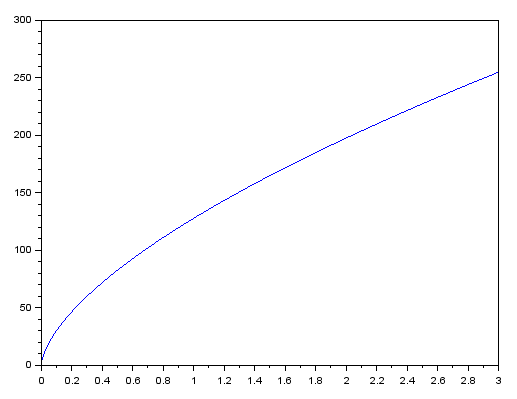
\includegraphics[height=6cm]{Fr-linear-azul}
    \label{figConceitoEixoA}
  }
  \quad %espaco separador
  \subfloat[Logarítmico]
  {
    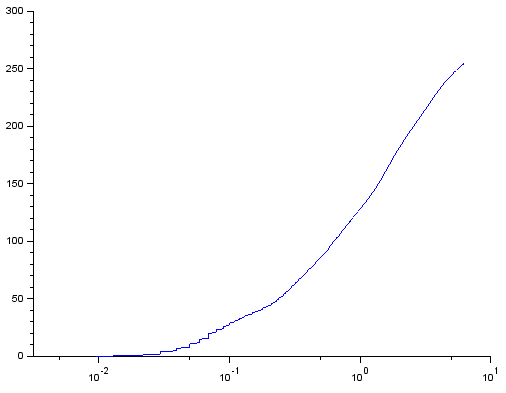
\includegraphics[height=6cm]{Fr-log-azul}
    \label{figConceitoEixoB}
  }
  \caption{Funções resposta e suas representações em diferentes eixos.}
  \label{figConceitoEixo}
\end{figure}

	A importância do eixo logarítmico para os métodos de geração de imagens HDR se dá por conta de uma suposição assumida por alguns dos autores. Segundo Mann \cite{mann} e Robertson \cite{robertson} a derivada da função resposta da câmera num eixo logarítmico possui relação direta com a confiabilidade que um pixel possui, i.e, quanto maior o valor de confiabilidade menor o ruído associado ao pixel. O cálculo da derivada do ponto de uma função em relação ao eixo logarítmico é dado pela seguinte equação:
	
\begin{align} \label{eqConceitoLog1}
          y^,_{log}(x) = \frac{dy}{dx}.\frac{x}{log(e)}
\end{align}

\section{Similaridade Bidirecional} \label{conceitoSimilaridadeBidirecional}
	A Similaridade Bidirecional \cite{simakov} é um método de maximização das similaridades entre dois sinais $S$(fonte) e $T$(destino), que se utiliza de um conjunto de fragmentos de ambos os sinais para definir a similaridade tanto em relação à sua coerência quanto à completude das informações.
	
	Uma imagem $T$ é dita coerente em relação a outra imagem $S$ quando todo fragmento $P_i$, pertencente a $T$, está contido em $S$. Por outro lado, se $T$ contém todos os fragmentos de $S$, então é dita completa em relação a $S$.
	
	O método maximiza a similaridade visual por meio da minimização da seguinte função:
	
\begin{align} \label{eqConceitoSimilaridade}
          d(S,T) = \frac{1}{N_S}\sum\limits_{P \subset S}{\underset{Q \subset T}{min}~D(P,Q)} + \frac{1}{N_T}\sum\limits_{Q \subset T}{\underset{P \subset S}{min}~D(Q,P)}
\end{align}

Onde
\begin{itemize}
	\item $N_S$ e $N_T$ são os números de fragmentos de $S$ e de $T$ respectivamente.
	\item $D(,)$ representa a distância, i.e., dissimilaridade entre dois fragmentos. 
\end{itemize} 
	

 \section{Relaxação de Gauss-Seidel} \label{conceitoGauss-Seidel}
	Consiste num método para resolução de sistemas de equações com múltiplas variáveis simultaneamente de forma iterativa. O método consiste em, a partir de valores especulados iniciais, inferir o valor de uma variável e com este valor encontrado, encontrar o valor da próxima variável. E assim prosseguir no método iterativo para todas as variáveis de maneira cíclica até atingir uma determinada condição de convergência. Mais informações sobre o método estão disponíveis na Referência \cite{livroCalculoNumerico}.
	

\section{Spline Cúbica} \label{conceitoSpline}

	Spline cúbica é um método de interpolação que possui como principal característica a geração de uma função contínua, com primeira e segunda derivadas também contínuas. A interpolação consiste em, dado um conjunto de pontos $S$ = $\{(x_i,y_i)\}$, obter uma função $y(x)$ que contenha todos estes pontos. Para isso considera-se que cada intervalo entre dois pontos consecutivos são funções polinomiais de terceiro grau. E a partir de premissas definidas em relação ao primeiro e ultimo ponto, é descoberto os valores das fuções de cada intervalo. Mais informações estão disponíveis na Referência \cite{livroCalculoNumerico}.
	
	
	
	